\documentclass[lettersize,journal]{IEEEtran}
\usepackage{amsmath,amsfonts}
\usepackage{algorithmic}
\usepackage{algorithm}
\usepackage{array}
\usepackage{booktabs}
\usepackage{multirow}
\usepackage[caption=false,font=normalsize,labelfont=sf,textfont=sf]{subfig}
\usepackage{textcomp}
\usepackage{stfloats}
\usepackage{url}
\usepackage{graphicx}
\usepackage{cite}
\usepackage{tikz}
\usetikzlibrary{arrows.meta, positioning, shapes.geometric}
\hyphenation{op-tical net-works semi-conduc-tor IEEE-Xplore}

\begin{document}

\title{CADENCE: Case-Grounded, Deliberation-Driven, and\\ Solver-Verified Architectural Decision-Making\\ with Large Language Models}

\author{Quang-Vinh~Dang
\thanks{Q.-V. Dang is with British University Vietnam, Hung Yen, Vietnam (e-mail: vinh.dq4@buv.edu.vn).}
\thanks{Manuscript submitted to the IEEE Transactions on Services Computing Special Issue on ``Large Language Models in Service-Oriented Ecosystems Design: Advances and Applications,'' 2026.}}

\markboth{IEEE Transactions on Services Computing, Special Issue on LLMs in Service-Oriented Ecosystems Design, 2026}%
{Dang: CADENCE: Solver-Verified Architectural Decision-Making with LLMs}

\maketitle

\begin{abstract}
Large language models (LLMs) are increasingly proposed as assistants for architectural decision-making in service-oriented systems, yet most existing approaches either generate an architecture decision record (ADR) from a single unconstrained LLM call, retrieve similar precedents without reconciling the competing quality-attribute concerns a real decision must balance, or debate among multiple agents without any formal check that the resulting decision is realizable within a bounded budget of architectural tactics. We present CADENCE, a four-stage algorithm combining (1) retrieval-augmented case-based reasoning over a corpus of real, mined ADRs, (2) knowledge-graph-grounded multi-agent deliberation in which each agent advocates for one ISO/IEC~25010-derived quality attribute, (3) constraint-solver-verified feasibility, encoded as a two-phase weighted MaxSAT/SMT problem in Z3 and repaired via an LLM-driven loop targeting the solver's uncovered-attribute signal (its unsatisfiable core is reported only as a supplementary diagnostic), and (4) a separate self-critique finalization pass blending a deterministic structural utility score with a qualitative LLM judgment. Unlike prior multi-agent architectural decision systems, whose agents occupy sequential functional roles and whose ``evaluation'' step is itself another LLM opinion, CADENCE's agents represent adversarial quality-attribute concerns and its feasibility check is a formal solver, not a second language model. We implement the full pipeline against a real corpus of 6{,}173 mined ADRs and evaluate it on two independently-sampled held-out sets ($N=3$ each, real end-to-end local-model wall-clock cost being the binding constraint on sample size) against four baselines forming an ablation ladder --- zero-shot generation, retrieval-only generation, multi-agent deliberation without solver verification, and CADENCE without self-critique --- on BERTScore, BLEU, ROUGE-1, and METEOR, together with two metrics only a solver-verified system can report at all: constraint-satisfaction rate and repair-loop convergence. Constraint satisfaction is 0\% and repair never converges before the iteration cap in every run, including when the repair loop is given its full design budget of two attempts --- an honest negative result at this sample size and configuration, which we diagnose mechanistically rather than soften. Against this, self-critique shows a modest but consistent positive signal: CADENCE with self-critique scores higher than the same pipeline without it on generation-quality metrics in 7 of 8 system-budget-metric comparisons, the only ablation in this evaluation where adding a stage helps rather than being flat. We separately find that surface n-gram metrics penalize CADENCE's deliberately terse, solver-parseable output relative to baselines prompted for open-ended prose, while BERTScore, a semantic-similarity metric insensitive to this length mismatch, remains comparable across all systems; we argue this is an asymmetry, not a quality gap, and discuss its implications for evaluating structured multi-stage LLM pipelines in general. Beyond our own re-implemented baselines, we further match our exact held-out items against a public replication package's own real, published generations from four frontier models, giving an external reference point our baselines alone cannot provide.
\end{abstract}

\begin{IEEEkeywords}
Large language models, architectural decision-making, architecture decision records, multi-agent systems, constraint solving, retrieval-augmented generation, self-critique, service-oriented architecture.
\end{IEEEkeywords}

\section{Introduction}

\IEEEPARstart{S}{ervice-oriented} systems accumulate architectural decisions continuously: how to scale a read-heavy service, whether to introduce a message queue, where to draw a service boundary, how to trade encryption overhead against latency. Each such decision commits a team to a set of consequences across multiple, frequently conflicting quality attributes --- performance against maintainability, scalability against cost, security against usability --- and each is, in practice, made under time pressure, with incomplete visibility into precedent, and without a systematic check that the chosen combination of architectural tactics is even mutually consistent within whatever operational budget the team can actually staff and afford. Architecture decision records (ADRs) exist precisely to make this reasoning explicit and reviewable, yet the discipline of writing one well --- surveying precedent, weighing competing quality attributes on their merits, and verifying that the resulting commitments do not silently exceed what the team can deliver --- is exactly the kind of effortful, multi-perspective reasoning that teams under delivery pressure are most likely to shortcut.

Large language models are a natural candidate to assist here, and a growing body of work has begun to explore LLM-assisted architectural decision-making and ADR generation. The most direct approaches prompt a single LLM, zero-shot or with light context, to draft a decision from a stated set of requirements~\cite{dhar2024llm}. A second line of work grounds generation in retrieval over real, mined ADR corpora, so that the model's output is anchored in precedent rather than invented from parametric knowledge alone~\cite{contextmatters2026}. A third line introduces multiple LLM agents into the process, most notably a four-agent pipeline of functional roles --- an Analyst, a Modeler, a Designer, and an Evaluator --- each handling a different phase of the decision~\cite{maad2025}. Each of these three lines of work solves part of the problem this paper is concerned with, but none solves all of it at once, and --- more importantly --- none of them can answer a question that matters for any decision with real operational consequences: \emph{is the decision the model just wrote actually feasible, given a bounded and explicit budget of architectural commitments the team can realistically execute?} A single LLM call has no mechanism to check this. Retrieval grounds the decision in precedent but does not reconcile competing quality-attribute demands against each other, let alone verify them formally. And a multi-agent pipeline whose final ``Evaluator'' step is itself another LLM call is still, ultimately, one model's opinion about another model's output --- persuasive, perhaps, but not a proof of anything.

This paper presents CADENCE, a four-stage algorithm for LLM-assisted architectural decision-making that is designed around this gap directly. CADENCE (1) retrieves precedent decisions from a real corpus of mined, human-authored ADRs via dense vector search, so that deliberation starts from what teams have actually decided before, not from a blank context window; (2) stages a bounded, structured multi-agent deliberation in which each agent is anchored to one ISO/IEC~25010-derived quality attribute --- performance, security, maintainability, scalability, and cost/operability --- and argues for the candidate decision that best serves its attribute, grounded in a knowledge graph of architectural tactics, so that the competing concerns a real decision must balance are represented explicitly and adversarially rather than folded into one model's undifferentiated judgment, with the graph's cross-attribute trade-off structure carried forward into Stage~3's feasibility check and Stage~4's utility scoring; (3) encodes the deliberated candidate's implied tactic commitments as a two-phase weighted MaxSAT/SMT problem and checks it with the Z3 theorem prover, and, if the encoding is infeasible under a caller-specified tactic budget, constructs a targeted repair prompt from the solver's uncovered-attribute signal (its unsatisfiable core, when available, is reported as a supplementary diagnostic rather than the repair driver) and issues it as a standalone repair call, iterating to a fixed cap and degrading gracefully with an explicit caveat if feasibility is never reached; and (4) finalizes the solver-verified decision through a separate self-critique pass that combines a deterministic structural utility score --- derived directly from which quality attributes the selected tactics actually cover, and what trade-offs they incur --- with a qualitative LLM judgment of the decision's remaining weaknesses, so that the system's own claimed confidence is never purely self-reported by the same reasoning process that produced the decision. Each stage exists to close a specific failure mode the others leave open: retrieval alone cannot reconcile competing quality attributes; deliberation alone cannot verify feasibility; and an unverified, unaudited decision cannot be trusted as final without an independent finalization pass.

We implement the complete CADENCE pipeline end-to-end against a real, publicly available corpus of 6{,}173 mined ADRs drawn from 882 open-source repositories~\cite{buchgeher2023adr}, and evaluate it against four baselines forming an ablation ladder, each adding exactly one stage over the previous one: zero-shot generation (no retrieval, no deliberation, no verification), retrieval-only generation (retrieval without deliberation or verification), multi-agent deliberation without solver verification (retrieval and deliberation only), and CADENCE without self-critique (adds Stage~3's solver-verified feasibility and repair loop, but not Stage~4). This ladder isolates retrieval's, deliberation's, solver verification's, and self-critique's contributions individually. We report the standard generation-quality metrics used in prior ADR-generation work --- BERTScore, BLEU, ROUGE-1, and METEOR --- against held-out, human-authored ground truth, alongside two metrics that only a solver-verified system can report at all: constraint-satisfaction rate and repair-loop convergence. Our results surface a methodologically important asymmetry: surface n-gram overlap metrics (ROUGE-1, METEOR) penalize CADENCE's deliberately terse, structured output --- terse by design, so that Stages 3 and 4 can parse it reliably --- relative to baselines prompted for open-ended prose closer in length to the reference ADRs, while BERTScore, a semantic-similarity metric far less sensitive to this length mismatch, remains comparable across all four systems. We report this honestly rather than letting a metric artifact of our own prompt design misrepresent the comparison, and we discuss what it implies for evaluating structured, multi-stage LLM pipelines whose intermediate representations are deliberately not free-form prose.

This work makes three contributions. First, we present CADENCE, to our knowledge the first architectural decision-making algorithm to combine real-corpus retrieval, adversarial quality-attribute-grounded multi-agent deliberation, formal constraint-solver verification with a solver-in-the-loop repair mechanism, and a separately-scored self-critique finalization stage. Second, we give a concrete construction for turning free-text, LLM-authored architectural deliberation into a solvable constraint-satisfaction instance, with one design choice empirically validated during development: a lexicographic, rather than weighted-sum, multi-objective optimization is required to make quality-attribute coverage strictly dominate trade-off avoidance regardless of caller-supplied weight magnitudes, a subtlety a naive encoding gets wrong (Section~\ref{sec:method-stage3}). Whether the full construction reliably reaches feasibility in practice is a separate, open empirical question our own small-sample evaluation (Section~\ref{sec:evaluation}) does not yet settle --- we report a fully-diagnosed negative result on that specific point rather than a positive one, and say so plainly. Third, we report a real, if small-sample, empirical evaluation against real baselines on a real corpus, and surface and explain a metric asymmetry (BERTScore versus surface n-gram overlap) that we believe generalizes to other structured, multi-stage LLM systems whose output is deliberately not free-form prose.

The remainder of this paper is organized as follows. Section~\ref{sec:related} positions CADENCE against the closest prior systems for LLM-assisted architectural decision-making and against the broader techniques it draws on. Section~\ref{sec:method} presents the CADENCE algorithm in full, stage by stage. Section~\ref{sec:evaluation} describes our experimental setup, baselines, metrics, and results. Section~\ref{sec:discussion} discusses limitations, threats to validity, and the metric-asymmetry finding. Section~\ref{sec:conclusion} concludes.

\section{Related Work}
\label{sec:related}

\subsection{LLM-Assisted Architectural Decision-Making}

Dhar et al.~\cite{dhar2024llm} demonstrate that a single LLM, prompted with a stated architectural problem, can produce a plausible ADR, but their approach neither retrieves precedent nor verifies the result against any formal notion of feasibility: the model's output is accepted as-is. Follow-on work from the same group frames ADR authoring as an explicit drafting process rather than one-shot generation~\cite{dhar2025drafting}, and a separate recent study evaluates LLMs specifically as \emph{detectors} of violations against already-recorded architectural decisions~\cite{su2026violations} --- a complementary, downstream concern (checking compliance with a decision already made) rather than assisting the decision itself. A complementary line of work treats the growing body of real, mined ADRs as a resource in its own right rather than a target for generation: large-scale mining studies of ADR adoption in open-source projects~\cite{buchgeher2023adr} establish both the raw corpus this paper's retrieval stage draws on and the empirical observation --- corroborated in our own corpus statistics --- that ADR adoption per repository is sparse, which any retrieval-based system must be designed to tolerate rather than assume away. Building on such corpora, retrieval-grounded generation work~\cite{contextmatters2026,contextmatters-zenodo} shows that conditioning an LLM's ADR generation on retrieved precedent measurably improves output quality over unconditioned generation, and explicitly frames the task this paper's held-out evaluation also uses: given only a decision's title, generate the body. This precedent motivates our own held-out query construction (Section~\ref{sec:evaluation}) and supplies both the retrieval-only baseline our evaluation compares against directly and the corpus itself. Neither line of work, however, reconciles multiple quality-attribute concerns against each other or checks feasibility formally --- both are gaps CADENCE is designed to close.

The closest prior system to CADENCE is MAAD~\cite{maad2025}, a four-agent architectural decision-making pipeline in which an Analyst, a Modeler, a Designer, and an Evaluator agent each handle one sequential phase of the decision process; a related paper from an overlapping author group targets the adjacent problem of generating the \emph{rationale} behind an already-made decision rather than the decision itself~\cite{zhou2025rationale}. MAAD and CADENCE share the premise that a single LLM call is insufficient and that multiple agents should participate in producing an architectural decision, but the two systems differ in three concrete, load-bearing ways. First, MAAD's agents occupy sequential \emph{functional} roles --- each agent does a different \emph{kind} of work at a different point in a pipeline --- whereas CADENCE's agents occupy simultaneous, \emph{adversarial} roles: every agent does the same kind of work (propose and critique a candidate decision) but from the standpoint of a different, often conflicting quality attribute, so that the tension between (for instance) a performance-motivated tactic and its maintainability cost is represented as an argument between agents rather than resolved silently inside one agent's internal reasoning. Second, MAAD's Evaluator is itself an LLM judge: it assesses the Designer's output using the same kind of model that produced it, so MAAD's final confidence signal is, ultimately, one language model's opinion of another's work. CADENCE's Stage~3 feasibility check is a formal constraint solver over an explicit tactic budget and quality-attribute coverage requirement; a decision either satisfies the encoded constraints or it does not, independent of any model's subjective assessment, and when it does not, the solver's uncovered-attribute signal gives the repair loop a structured, specific target rather than generic revision instructions (the unsatisfiable core is also reported, as a supplementary diagnostic). Third, CADENCE's retrieval stage is grounded in a large, real, citable corpus of mined ADRs from open-source practice, giving deliberation a case-based starting point that MAAD's requirements-only formulation does not provide. We discuss MAAD further, and compare against a solver-free multi-agent ablation modeled directly on this difference, in Section~\ref{sec:evaluation}. Table~\ref{tab:relatedwork} summarizes this positioning against the three closest prior systems.

\begin{table*}[t]
\caption{Positioning Against the Closest Prior LLM-Assisted Architectural Decision-Making Systems\label{tab:relatedwork}}
\centering
\footnotesize
\setlength{\tabcolsep}{3pt}
\begin{tabular}{@{}
  >{\raggedright\arraybackslash}p{1.05in}
  >{\centering\arraybackslash}p{0.5in}
  >{\centering\arraybackslash}p{0.5in}
  >{\raggedright\arraybackslash}p{1.65in}
  >{\raggedright\arraybackslash}p{1.35in}
  >{\raggedright\arraybackslash}p{1.15in}
@{}}
\toprule
System & Real-corpus retrieval & Multi-agent & Agent roles & Formal solver verification & Separate critique stage \\
\midrule
Dhar et al.~\cite{dhar2024llm}            & No  & No             & ---                                                                    & No             & No \\
Context Matters~\cite{contextmatters2026} & Yes & No             & ---                                                                    & No             & No \\
MAAD~\cite{maad2025}                      & No  & Yes (4 agents) & Sequential functional roles (Analyst / Modeler / Designer / Evaluator) & No (LLM judge) & No (folded into pipeline) \\
\textbf{CADENCE (this work)}              & Yes & Yes            & Simultaneous adversarial quality-attribute advocates                  & \textbf{Yes} (Z3 weighted MaxSAT/SMT + repair loop) & \textbf{Yes} (distinct utility-scoring pass) \\
\bottomrule
\end{tabular}
\end{table*}

\subsection{LLMs for Service-Oriented and Microservice Architecture}

A recent review of LLMs across the service-computing lifecycle explicitly names architectural decision support an open direction, not a solved one~\cite{kumara2026llm4soc} --- the two concrete service-oriented design systems that exist target a different point on that lifecycle: one recommends monolith-to-microservice decompositions via contrastive learning alongside an LLM~\cite{sellami2025microservice}, the other synthesizes candidate microservice architectures directly from textual requirements~\cite{albuquerque2026microservice}. Both decompose or synthesize a service \emph{topology}; neither decides and justifies one architectural \emph{commitment} against competing quality-attribute concerns the way CADENCE does, so the gap the review names is still open for this paper's special-issue theme specifically, not just in general.

\subsection{LLM--Solver Integration}

Combining LLMs with formal solvers to check or verify what a model proposes is an active area outside the architecture domain: representative approaches translate natural-language problems into a formal logical representation and dispatch it to a symbolic solver so that the solver, not the LLM, is responsible for the deductive step~\cite{pan2023logiclm}, and closely related work verifies LLM-authored natural-language proofs by first compiling them into a checkable formal representation~\cite{olausson2023linc}. More recent work bridges LLMs and symbolic solvers directly through the Model Context Protocol, giving a model a structured tool interface to a solver rather than a one-shot translation step~\cite{szeider2025mcpsolver}, and, closest in spirit to CADENCE's Stage~3, one planning system explicitly drives an LLM repair loop from a Z3 solver's unsatisfiable core when a proposed plan is infeasible~\cite{hao2024planningz3} --- the same solver-in-the-loop repair pattern this paper applies to architectural tactic feasibility rather than task planning. These techniques target logical inference, formal proof checking, and classical planning; CADENCE applies the same underlying pattern --- let the LLM produce a candidate, let a solver check it, and feed the solver's failure signal back to the LLM for repair --- to a different, softer verification target: whether a candidate architectural decision's implied tactic commitments are jointly satisfiable within an explicit resource budget and quality-attribute coverage requirement, encoded as weighted MaxSAT/SMT rather than propositional or first-order logic or a planning domain. To our knowledge, no prior work applies solver-in-the-loop verification specifically to architectural trade-off feasibility; we cite this literature as prior art for the general LLM-plus-solver \emph{technique}, not as prior work on the specific \emph{application}.

\subsection{Multi-Agent Deliberation and Self-Critique with LLMs}

Multi-agent debate among LLM instances has been shown to improve factual accuracy and reasoning quality over single-model generation by exposing a claim to independent critique before it is accepted~\cite{duetal2023debate}, an effect corroborated by independent work showing debate encourages divergent thinking that a single model's self-reflection alone does not reliably produce~\cite{liang2024divergent}, and extended to using multi-agent debate itself as an evaluation mechanism for other models' outputs~\cite{chan2024chateval}. CADENCE's Stage~2 deliberation applies this general finding to a domain-specific structure: rather than generic, undifferentiated debate, each agent's role and critique perspective is fixed to one ISO/IEC~25010 quality attribute and grounded in a shared knowledge graph of architectural tactics, so the debate is anchored to a concrete, checkable tactic vocabulary rather than open-ended argument, with the graph's documented cross-attribute trade-offs consumed downstream by Stage~3's feasibility check and Stage~4's utility scoring rather than argued over directly within Stage~2 itself. Separately, self-refinement work shows that a model can improve its own output by critiquing and revising it in a subsequent pass, without external supervision~\cite{madaan2023selfrefine}, and verbal-reinforcement approaches extend this across multiple attempts using episodic memory of past failures~\cite{shinn2023reflexion}. This literature is not uniformly optimistic, however: a widely-cited negative result finds that LLMs prompted to self-correct their own reasoning \emph{without external feedback} frequently fail to improve, and can even degrade an already-correct answer~\cite{huang2024selfcorrect} --- a finding we take seriously and address directly in Stage~4's design (Section~\ref{sec:method-stage4}) and in our threats-to-validity discussion (Section~\ref{sec:discussion}). CADENCE's Stage~4 draws on the self-refinement idea but departs from both strands in one respect we consider important for high-stakes decisions: the self-critique pass is not a further revision of the same reasoning chain in isolation, but an independently-scored finalization that combines a deterministic structural component --- computed directly from Stage~3's solver output, not re-derived by an LLM --- with the qualitative LLM judgment, so the system's final confidence is never solely the same model marking its own homework without external (solver-verified) grounding.

\subsection{Case-Based Reasoning and Retrieval-Augmented Generation}

Case-based reasoning --- solving new problems by adapting solutions to similar past problems --- is a natural fit for architectural decision-making, since real decisions are rarely made from first principles but from precedent, convention, and prior experience; recent work formalizes how case-based reasoning's classical case-retrieve-reuse-revise cycle maps onto LLM agents specifically~\cite{hatalis2025cbrllm}, and a concrete instantiation combines case-based retrieval with generation for a different high-stakes domain (legal question answering), demonstrating the pattern's applicability beyond architecture~\cite{wiratunga2024cbrrag}. CADENCE's Stage~1 operationalizes this classical idea with dense vector retrieval over a real ADR corpus rather than a hand-curated case base, following the same retrieval-augmented generation methodology increasingly used to ground LLM generation in verifiable external evidence more broadly~\cite{lewis2020rag}, including within software engineering specifically, where a recent survey catalogs repository-level retrieval strategies for code generation that parallel this paper's corpus-level retrieval for architectural precedent~\cite{tao2025ragcode}. The architectural tactics that structure CADENCE's knowledge graph and constraint encoding --- caching, connection pooling, horizontal scaling, circuit breakers, and the like, together with their well-known cross-quality-attribute trade-offs --- are an original, structured synthesis informed by and in the spirit of the established software architecture tactics catalog~\cite{bass2021saip}, not a reproduction of its specific text, which this paper's Stage~2/3 machinery operationalizes into a form an LLM-driven deliberation and a formal solver can both act on.

\section{The CADENCE Algorithm}
\label{sec:method}

\subsection{Problem Formulation and Overview}

CADENCE takes as input a natural-language decision context $c$ (the requirements and situational description a real ADR's ``Context'' section would state) and a set of required quality attributes $Q = \{q_1, \ldots, q_5\} \subseteq \{\textit{performance}, \textit{security}, \textit{maintainability}, \textit{scalability}, \textit{cost\_operability}\}$, the ISO/IEC~25010-derived taxonomy fixed for this work. It produces a finalized, provenance-complete architectural decision record: a decision statement, a rationale, a per-quality-attribute utility score, a feasibility verdict with the selected architectural tactics and any residual gaps, and a full transcript of the precedents consulted, the agent positions debated, and the repair iterations taken to reach the final candidate. The four stages --- retrieval, deliberation, solver verification with repair, and self-critique finalization --- execute in sequence, each consuming the previous stage's output and each addressing a distinct failure mode the others do not cover. Figure~\ref{fig:pipeline} shows the overall flow, and Algorithm~\ref{alg:cadence} gives it formally.

\begin{figure*}[t]
\centering
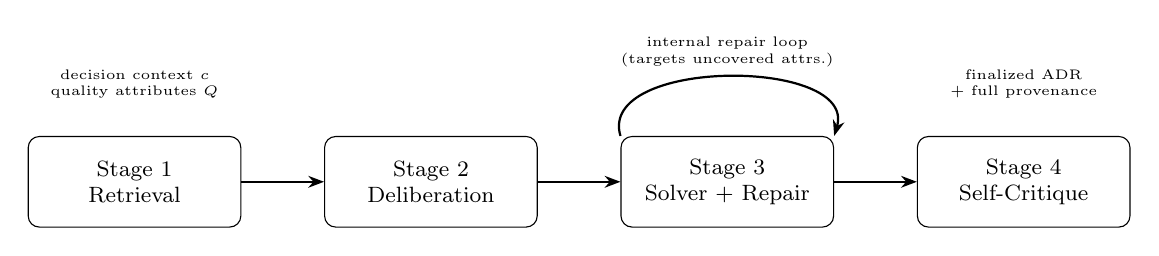
\begin{tikzpicture}[
  stage/.style={draw, rounded corners, minimum width=2.7cm, minimum height=1.15cm, align=center, font=\footnotesize},
  arr/.style={-{Stealth[length=2mm]}, thick},
  node distance=1.05cm
]
\node[stage] (retrieval) {Stage 1\\Retrieval};
\node[stage, right=of retrieval] (delib) {Stage 2\\Deliberation};
\node[stage, right=of delib] (solver) {Stage 3\\Solver + Repair};
\node[stage, right=of solver] (critique) {Stage 4\\Self-Critique};

\draw[arr] (retrieval) -- (delib);
\draw[arr] (delib) -- (solver);
\draw[arr] (solver) -- (critique);

\draw[arr] (solver.north west) .. controls +(-0.3,1.0) and +(0.3,1.0) .. (solver.north east)
  node[midway, above, font=\tiny, align=center] {internal repair loop\\(targets uncovered attrs.)};

\node[above=0.35cm of retrieval, font=\tiny, align=center] {decision context $c$\\quality attributes $Q$};
\node[above=0.35cm of critique, font=\tiny, align=center] {finalized ADR\\+ full provenance};
\end{tikzpicture}
\caption{The CADENCE pipeline. Each stage consumes the previous stage's output; Stage~3's repair loop is internal to Stage~3 --- it never re-enters Stage~2's multi-agent deliberation --- and issues a standalone repair call driven by the solver's uncovered-attribute signal (with the unsatisfiable core reported only as a supplementary diagnostic), iterating to a fixed cap before Stage~4 finalizes the decision.\label{fig:pipeline}}
\end{figure*}

\begin{algorithm}[t]
\caption{CADENCE}
\label{alg:cadence}
\begin{algorithmic}[1]
\REQUIRE context $c$, quality attributes $Q$, tactic budget $B$, tactic catalog with graph $G$, max deliberation rounds $R$, max repair iterations $K$
\ENSURE finalized decision with provenance
\STATE $P \gets \textsc{Retrieve}(c)$ \COMMENT{Stage 1: top-$k$ precedents}
\STATE $(d, r) \gets \textsc{Deliberate}(c, P, Q, G, R)$ \COMMENT{Stage 2: bounded multi-agent debate}
\STATE $i \gets 0$; $\mathit{best} \gets \bot$
\LOOP
  \STATE $\mathit{res} \gets \textsc{CheckFeasibility}(d, Q, B, G)$ \COMMENT{Stage 3, Phase 1+2}
  \IF{$\mathit{best} = \bot$ \textbf{or} $|\mathit{res}.\mathit{covered}| > |\mathit{best}.\mathit{res}.\mathit{covered}|$}
    \STATE $\mathit{best} \gets (\mathit{res}, d, r)$ \COMMENT{track highest-coverage attempt seen so far}
  \ENDIF
  \IF{$\mathit{res}.\mathit{feasible}$ \textbf{or} $i = K$}
    \STATE \textbf{break} \COMMENT{degrade gracefully with a caveat if infeasible}
  \ENDIF
  \STATE $(d, r) \gets \textsc{Repair}(d, \mathit{res}.\mathit{uncovered}, B)$ \COMMENT{standalone LLM repair call, targets uncovered attributes}
  \STATE $i \gets i + 1$
\ENDLOOP
\STATE $(\mathit{res}, d, r) \gets \mathit{best}$ \COMMENT{use the best attempt seen, not necessarily the last}
\STATE $u \gets \textsc{StructuralUtility}(\mathit{res}, G)$ \COMMENT{Stage 4, deterministic}
\STATE $q \gets \textsc{QualitativeCritique}(d, r, Q)$ \COMMENT{Stage 4, separate LLM pass}
\RETURN $\textsc{Finalize}(d, r, u, q, \mathit{res}, P)$
\end{algorithmic}
\end{algorithm}

\subsection{Stage 1: Retrieval-Augmented Case-Based Reasoning}

Stage 1 embeds the decision context $c$ with a sentence-embedding model and retrieves the $k$ nearest precedent ADRs, by cosine similarity, from a dense vector index built over the full corpus of $6{,}173$ real, mined ADRs (Section~\ref{sec:evaluation}). Each corpus record is parsed leniently from its source Markdown file --- real-world ADR filenames and internal structure are inconsistent across repositories, so the parser extracts only a title and the full raw body text rather than assuming any fixed section schema. Retrieval returns the top-$k$ precedent records, whose titles are passed into Stage~2 as grounding context for every deliberation agent; when Stage~1 is used inside a held-out evaluation, the query record's own ground-truth ADR is explicitly excluded from its own retrieval results to prevent leakage.

\subsection{Stage 2: Knowledge-Graph-Grounded Multi-Agent Deliberation}

Stage 2 instantiates one \texttt{QualityAttributeAgent} per required quality attribute in $Q$. Each agent is grounded in a knowledge graph $G$ built from a hand-curated catalog of 26 architectural tactics spanning the five quality attributes (5 or 6 tactics per attribute; Table~\ref{tab:tactics} lists the full catalog), where each tactic node has a directed \emph{supports} edge to the quality attribute it primarily serves and directed \emph{trade-off} edges, annotated with a natural-language explanation, to every other quality attribute it is known to burden --- for instance, \emph{caching} supports \emph{performance} but trades off against \emph{maintainability} via cache-invalidation complexity, and \emph{authentication} supports \emph{security} but trades off against both \emph{performance} (per-request verification latency) and \emph{cost\_operability} (identity-infrastructure upkeep), as Figure~\ref{fig:kg-excerpt} depicts. Given the decision context and Stage~1's retrieved precedents, each agent proposes a candidate decision serving its own attribute using $G$'s \emph{supports} edges to select from its attribute's own tactic vocabulary, and may critique the candidates proposed by other agents; $G$'s \emph{trade-off} edges are consumed downstream, by Stage~3's feasibility optimization and Stage~4's structural utility score, rather than injected directly into Stage~2's agent prompts. Deliberation proceeds for a bounded number of rounds (\texttt{max\_rounds}, an algorithm parameter) after which an orchestrator synthesizes the debate into a single converged candidate decision and rationale.

\begin{figure}[t]
\centering
\resizebox{\columnwidth}{!}{%
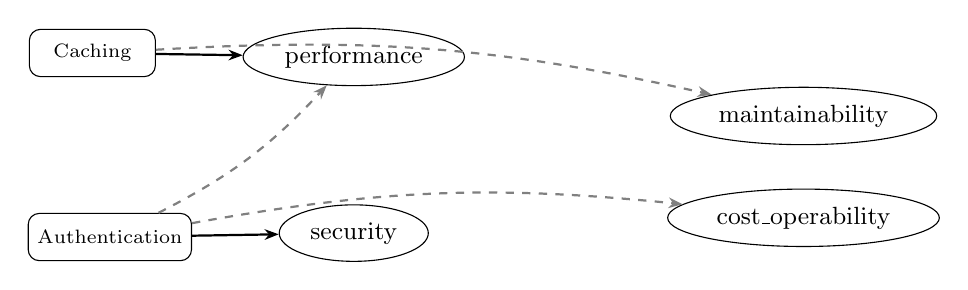
\begin{tikzpicture}[
  qa/.style={draw, ellipse, minimum width=1.55cm, minimum height=0.7cm, align=center, font=\small},
  tac/.style={draw, rounded corners, minimum width=1.6cm, minimum height=0.6cm, align=center, font=\scriptsize},
  supp/.style={-{Stealth[length=1.8mm]}, thick},
  trad/.style={-{Stealth[length=1.8mm]}, dashed, thick, gray},
  node distance=0.55cm and 1.15cm
]
\node[qa] (perf) {performance};
\node[qa, below=1.5cm of perf] (sec) {security};
\node[qa, right=2.6cm of perf, yshift=-0.75cm] (maint) {maintainability};
\node[qa, below=0.55cm of maint] (cost) {cost\_\allowbreak operability};
\node[tac, left=1.1cm of perf, yshift=0.05cm] (caching) {Caching};
\node[tac, left=1.1cm of sec, yshift=-0.05cm] (auth) {Authentication};

\draw[supp] (caching) -- (perf);
\draw[trad] (caching) to[bend left=8] (maint);
\draw[supp] (auth) -- (sec);
\draw[trad] (auth) to[bend right=10] (perf);
\draw[trad] (auth) to[bend left=8] (cost);
\end{tikzpicture}%
}
\caption{Excerpt of knowledge graph $G$: solid arrows are \emph{supports} edges, dashed gray arrows are \emph{trade-off} edges. Only 2 of the catalog's 26 tactics and 4 of its 5 quality attributes are shown for legibility.\label{fig:kg-excerpt}}
\end{figure}

\begin{table*}[t]
\caption{The 26-Tactic Catalog Grounding Stage 2's Knowledge Graph $G$\label{tab:tactics}}
\centering
\footnotesize
\setlength{\tabcolsep}{4pt}
\begin{tabular}{@{}
  >{\raggedright\arraybackslash}p{0.42in}
  >{\raggedright\arraybackslash}p{1.7in}
  >{\raggedright\arraybackslash}p{2.55in}
  >{\centering\arraybackslash}p{0.45in}
@{}}
\toprule
QA & Tactic & Primary Effect & \#TOs \\
\midrule
\multirow{5}{*}{Perf.}
 & Caching & Store frequently-accessed results to avoid recomputation or I/O & 1 \\
 & Connection pooling & Reuse expensive connections instead of opening one per request & 1 \\
 & Async.\ processing via message queues & Decouple slow work from the request path via a queue & 2 \\
 & Data denormalization & Duplicate data to avoid expensive joins/cross-service calls & 1 \\
 & Read-through/write-behind access & Batch or defer writes, prefetch reads & 1 \\
\midrule
\multirow{6}{*}{Sec.}
 & Authentication & Verify caller identity before granting access & 2 \\
 & Fine-grained authorization & Restrict operations to callers' specific permissions & 1 \\
 & Encryption in transit/at rest & Protect data from interception or disk-level access & 2 \\
 & Rate limiting / throttling & Cap load a single caller can place on the system & 1 \\
 & Least-privilege service boundaries & Give services only needed access, isolate blast radius & 1 \\
 & Input validation at trust boundaries & Reject malformed/malicious input as early as possible & 1 \\
\midrule
\multirow{5}{*}{Maint.}
 & Modular decomposition by capability & Split system along business boundaries & 2 \\
 & Versioned API contracts & Evolve boundaries without breaking consumers & 1 \\
 & Automated regression test suite & Catch behavioral regressions before production & 1 \\
 & Centralized structured logging & Make system behavior inspectable for debugging & 2 \\
 & Dependency injection / IoC & Decouple components from concrete dependency impls & 1 \\
\midrule
\multirow{5}{*}{Scal.}
 & Horizontal scaling, stateless instances & Add identical instances instead of growing one & 2 \\
 & Database sharding & Partition data across DB instances by shard key & 2 \\
 & Event-driven architecture & Components communicate via events, not sync calls & 2 \\
 & Auto-scaling infrastructure & Add/remove capacity per observed load automatically & 1 \\
 & Read replicas & Serve read traffic from replicated data copies & 1 \\
\midrule
\multirow{5}{*}{Cost}
 & Managed cloud services & Use a vendor-operated service instead of self-hosting & 2 \\
 & Infrastructure as code & Define infrastructure declaratively for reproducibility & 0 \\
 & Multi-tenancy & Share infrastructure across tenants, not per-tenant & 2 \\
 & Serverless / FaaS deployment & Pay only for actual invocation time & 2 \\
 & Circuit breaker for dependencies & Stop calling a failing dependency instead of retrying & 1 \\
\bottomrule
\end{tabular}

\vspace{2pt}
\footnotesize \#TOs: number of \emph{trade-off} edges the tactic carries to other quality attributes in $G$ (0--2 in this catalog); QA: the quality attribute the tactic's \emph{supports} edge targets. Full trade-off targets and natural-language rationale for each edge are in \texttt{src/deliberation/knowledge\_graph.py} (see Data and Code Availability).
\end{table*}

Synthesis is the stage's most format-fragile step: it asks the underlying LLM to emit a structured \texttt{CANDIDATE}/\texttt{RATIONALE} response that Stage~3 can parse deterministically. In practice, real small-model output deviates from any single expected format in ways a fixed parser cannot fully anticipate in advance (Section~\ref{sec:method-robustness}); the orchestrator therefore retries the same synthesis prompt up to three times on a parse failure before surfacing an error, since generation is stochastic and a differently-sampled retry frequently self-corrects a formatting slip that a hand-written regex extension would not have anticipated.

\subsection{Stage 3: Constraint-Solver-Verified Feasibility with Repair Loop}
\label{sec:method-stage3}

Stage 2's converged candidate is free text: a human-readable decision and rationale, not a structured commitment a solver can reason about directly. Stage 3 first extracts which of the 26 catalog tactics the candidate text actually mentions, via fuzzy word-stem overlap against each tactic's name, giving a set of Boolean decision variables $\{t_1, \ldots, t_m\}$, one per mentioned tactic. It then checks feasibility in two phases against the Z3 SMT solver.

\emph{Phase 1 (strict feasibility).} A budget constraint $\sum_i t_i \leq B$ (a caller-specified tactic budget $B$) and, for every required quality attribute $q \in Q$, a coverage constraint $\bigvee_{i \,:\, \mathrm{supports}(t_i) = q} t_i$ (at least one selected tactic must support $q$) are asserted with \texttt{assert\_and\_track}, so that if the instance is unsatisfiable, Z3 returns an \emph{unsatisfiable core}: the specific subset of constraints jointly responsible for infeasibility. This core is a genuinely useful, but not necessarily complete, diagnostic --- Z3's core-extraction semantics can name only one of several symmetric zero-coverage attributes as blocking, omitting others that are equally unsatisfied --- so Stage~3 does not treat it as authoritative.

\emph{Phase 2 (best-effort optimized selection).} A separate \texttt{Optimize} instance re-asserts the budget constraint and searches for the tactic selection that jointly (a) maximizes how many required quality attributes are covered and (b) minimizes the caller-weighted cost of the trade-offs incurred by the selected tactics, always returning a concrete selection even when Phase~1 found the instance strictly infeasible. These two objectives are declared under Z3's \texttt{priority="lex"} lexicographic mode as separate \texttt{add\_soft} groups, rather than combined into one weighted-sum objective --- a distinction we verified matters empirically. An earlier, weighted-sum formulation used a single large constant to bias coverage above trade-off cost, but because trade-off weights are caller-supplied with no upper bound, a tactic selection accumulating enough trade-off weight could mathematically outvote a required attribute's coverage regardless of the bias constant's size (a concrete repro during development: four trade-offs at weight 300 each outweighed a coverage bias of 1000). Lexicographic priority makes quality-attribute coverage strictly dominate trade-off avoidance independent of weight magnitude, which we consider the only encoding that is safe for caller-supplied weights whose scale cannot be bounded in advance. The resulting \texttt{covered\_quality\_attributes} / \texttt{uncovered\_quality\_attributes} split from this phase, not Phase~1's unsat core, is therefore the sound and complete signal of what still needs fixing.

If Phase~1 finds the instance infeasible, Stage~3 constructs a repair prompt that names, for every uncovered quality attribute, the concrete catalog tactics that would cover it, and asks the LLM to revise the candidate within the same tactic budget. This is re-checked against the solver, and the loop iterates up to \texttt{max\_repair\_iterations} times, tracking the best (highest-coverage) attempt seen across iterations. If the budget is never satisfiable within the iteration cap, Stage~3 returns the best attempt found together with an explicit caveat rather than either silently accepting an infeasible decision or discarding an otherwise-reasonable candidate; a transient LLM or parse failure during any individual repair attempt is treated as a reason to try the next iteration, not as a reason to abort the loop.

\subsection{Stage 4: Self-Critique Finalization}
\label{sec:method-stage4}

Stage 4 combines two independently-computed signals into each quality attribute's final utility score. The \emph{structural} component is deterministic: for a given attribute $q$, it is $1.0$ if $q$ is among the solver-verified decision's covered attributes, minus a fixed penalty of $0.2$ for every incoming trade-off edge from a selected tactic onto $q$ in $G$, floored at $0.0$. This component depends only on Stage~3's already-verified output and involves no further LLM call. The \emph{qualitative} component is a single LLM pass that scores every required attribute on a 0--10 scale and flags any residual weakness in the finalized decision, given the full decision, rationale, and attribute list in one call; parsing this response uses a three-tier matcher --- a strict same-line pattern tried first, a tolerant same-line fallback second, and a heading-section fallback third for responses that state an attribute as its own heading line with the field on a separate, unlabeled line (Section~\ref{sec:method-robustness}) --- so that a loose regex cannot lock onto a prose preamble instead of the real scored line further down the response, and the call is retried up to three times on a parse failure for the same reason Stage~2's synthesis call is. The two components are combined as $\mathrm{combined}_q = 0.5 \cdot \mathrm{structural}_q \cdot 10 + 0.5 \cdot \mathrm{qualitative}_q$, and the overall decision utility is the mean combined score across all required attributes. The finalized output --- the \texttt{FinalADR} --- carries this scoring together with full provenance: which precedents were retrieved, the complete per-agent deliberation transcript, which tactics were selected and by which repair iteration, and any solver caveat, so the decision is auditable end-to-end rather than presented as an opaque final answer.

\subsection{Implementation Robustness: Parsing Real, Stochastic LLM Output}
\label{sec:method-robustness}

A structured-output prompt's hand-written happy-path parser reliably breaks against a real, deployed small language model, and our development process surfaced this repeatedly and concretely rather than as a theoretical concern. Running the full pipeline end-to-end against Qwen2.5-1.5B-Instruct, the reproducible local backbone used throughout this work's experiments, produced six distinct real formatting deviations across Stages~2--4, summarized in Table~\ref{tab:deviations}.

\begin{table}[t]
\caption{Six Real LLM Output-Format Deviations Encountered\label{tab:deviations}}
\centering
\footnotesize
\setlength{\tabcolsep}{3pt}
\begin{tabular}{@{}
  >{\centering\arraybackslash}p{0.15in}
  >{\raggedright\arraybackslash}p{1.55in}
  >{\raggedright\arraybackslash}p{1.65in}
@{}}
\toprule
\# & Deviation & Resolved by \\
\midrule
1 & Extra descriptor word (``Candidate Decision:'' for ``Candidate:'') & Tolerant same-line parser \\
2 & Non-literal ``no weakness'' (``None identified'' for literal ``none'') & Tolerant same-line parser \\
3 & Fraction-style score (``8/10''), this model's \emph{default} 0--10 answer & Tolerant same-line parser \\
4 & Prose preamble a loose regex could lock onto instead of the real line & Tolerant same-line parser \\
5 & Genuine word substitution (``Candidacy:'' for ``Candidate:''), unanticipatable by regex tolerance & Bounded retry (2--3 attempts) \\
6 & Attribute-as-heading structure: attribute on its own heading line, field unlabeled on a later line & Third parser tier (heading-section fallback) \\
\bottomrule
\end{tabular}
\end{table}

The first four are addressable by a sufficiently tolerant same-line parser. The fifth is not, and its discovery is what motivated this work's general strategy of pairing every structured-output prompt with a bounded retry (two to three attempts) of the identical prompt on a parse failure, rather than continuing to special-case wording variants indefinitely; because generation is stochastic, a differently-sampled retry frequently self-corrects a formatting slip the parser did not anticipate, and Stages~2, 3, and 4 all apply this pattern. The sixth, discovered later during the real scaled evaluation run reported in Section~\ref{sec:evaluation} (e.g.\ \texttt{**Performance**} followed, several lines later, by \texttt{**Score:** 9/10} with no attribute name on that line at all), shows retry's limit: it exhausted all three attempts, because it was not a stochastic one-off a differently-sampled retry could route around, but a genuinely different \emph{structure} no same-line pattern, however tolerant, could ever match --- fixing it required a third parser tier (Section~\ref{sec:method-stage4}) that locates an attribute's heading line and then searches only the bounded section up to the next attribute's heading for an unlabeled field. We report this not as a footnote but as a methodological finding in its own right: any system that asks an LLM for structured intermediate output that a downstream deterministic component must consume --- as any solver-verified pipeline necessarily does --- should validate its parser against real, repeated model output before trusting it in an unattended run, should treat bounded retry as the general-purpose fix for wording variation, and should expect that retry alone is not sufficient: a genuinely new structural format, not just a wording variant, will eventually require a genuinely new parser tier, and finding out which one occurred requires actually running the real pipeline, not reasoning about the prompt in advance.

\subsection{Worked Example}
\label{sec:worked-example}

To make the four stages concrete rather than only described in the abstract, this section walks through one real, complete run of the pipeline reported verbatim from the actual implementation (\texttt{scripts/run\_worked\_example.py} in the released artifact) --- illustrative, not an evaluation data point; the quantitative claims of this paper come from Section~\ref{sec:evaluation}'s held-out runs, not from this single example.

\textbf{Context:} ``Our service-oriented system's order-processing service is experiencing 10x read traffic growth from a new mobile client. Requirements: keep p99 read latency low, keep the change operable by a small team, and avoid introducing new categories of security risk.''

\textbf{Stage 1} retrieves three real precedents from the corpus: \emph{``Use message broker for asynchronous messaging,''} \emph{``[0001] Server Architecture,''} and \emph{``Use JSON Web Token (`JWT') for authenticating inter-service API requests.''}

\textbf{Stage 2} runs two rounds across the five agents (propose, then critique), ten positions in total. The \emph{performance} agent's propose-round position opens: ``it is crucial to leverage proven strategies that minimize impact on the architecture... By using a message queue (e.g., RabbitMQ), we decouple the read operations from the main application server,'' while the \emph{security} agent's propose-round position independently argues for JWT authentication, encryption in transit and at rest, and rate limiting. In round 2, the \emph{cost\_operability} agent's critique flags a real cross-attribute tension the others' proposals introduced: ``Adding a message broker for asynchronous messaging increases network overhead and introduces latency. This could affect real-time interactions.'' The orchestrator synthesizes these into one converged candidate naming (among others) asynchronous message-queue processing, event-driven architecture, and serverless deployment.

\textbf{Stage 3} extracts three catalog tactics from that candidate --- \emph{asynchronous processing via message queues}, \emph{event-driven architecture}, and \emph{serverless/FaaS deployment} --- covering \emph{performance}, \emph{scalability}, and \emph{cost\_operability}, but not \emph{maintainability} or \emph{security}. Under $B=4$ this is a concrete, real instance of exactly the mechanism Section~\ref{sec:evaluation} diagnoses in aggregate: one tactic slot remained within budget, but the deliberated candidate's text never named a fourth, security- or maintainability-covering tactic for the extractor to find. Both repair attempts fail to close the gap, and Stage~3 returns the best-effort selection with an explicit caveat: ``Could not find a decision covering all required quality attributes within a budget of 4 tactics after 2 repair attempt(s). Best effort covers [`cost\_operability', `performance', `scalability'] but leaves [`maintainability', `security'] unaddressed.''

\textbf{Stage 4} finalizes the decision --- ``Implement a microservices-based architecture using a message queue for communication between services, an event sourcing database for persistent data storage, and serverless cloud functions for real-time processing and analytics'' --- and scores it per attribute (Table~\ref{tab:worked-example}), flagging a concrete, specific weakness for each rather than a generic caveat (e.g., for \emph{security}: ``serverless functions... still have inherent risks like function timeout limits and lack of direct control over execution environment''). The two uncovered attributes' structural components are correctly $0.0$, dragging their combined scores down even where the qualitative pass alone would have scored the prose favorably --- exactly the blending Section~\ref{sec:method-stage4} argues for: an uncovered attribute cannot be masked by confident-sounding text.

\begin{table}[t]
\caption{Worked Example: Per-Attribute Utility Scores (Overall: 6.6/10)\label{tab:worked-example}}
\centering
\footnotesize
\begin{tabular}{@{}lccc@{}}
\toprule
Quality Attribute & Structural & Qualitative & Combined \\
\midrule
Performance       & 0.8 & 8.0 & 8.0 \\
Security          & 0.0 & 9.0 & 4.5 \\
Maintainability   & 0.0 & 7.0 & 3.5 \\
Scalability       & 1.0 & 8.0 & 9.0 \\
Cost/Operability  & 1.0 & 6.0 & 8.0 \\
\bottomrule
\end{tabular}
\end{table}

\section{Evaluation}
\label{sec:evaluation}

\subsection{Corpus and Experimental Setup}

We evaluate against the ``Context Matters'' replication package~\cite{contextmatters-zenodo} (Zenodo, DOI:~10.5281/zenodo.18370195), derived from the same mining study that provides Stage~1's retrieval corpus~\cite{buchgeher2023adr}. The package's own \texttt{dataset\_index.json} catalogs 954 repository folders with an extraction-confidence status each (Table~\ref{tab:corpus-status}); after parsing, the 882 folders that contain at least one accessible Markdown file yield 6{,}173 individual ADR files (median 4, mean 7.00, maximum 129 per repository, confirming the corpus's documented per-repository sparsity) --- the remaining 72 catalogued folders have no accessible file at all (\texttt{Repo Inaccessible} or \texttt{Doubt (no repo dir)}) and contribute nothing to either count. We restrict our held-out evaluation set to the 750 folders marked \texttt{Verified}, so that ground-truth quality is not itself a confound.

\begin{table}[t]
\caption{Corpus Extraction-Confidence Breakdown (\texttt{dataset\_index.json}, 954 catalogued folders)\label{tab:corpus-status}}
\centering
\footnotesize
\begin{tabular}{@{}lc@{}}
\toprule
Status & Folders \\
\midrule
Verified & 750 \\
Doubt (name sequence) & 96 \\
Repo Inaccessible & 40 \\
Doubt (no repo dir) & 33 \\
Doubt (missing file) & 30 \\
Doubt (file contents) & 5 \\
\midrule
Total & 954 \\
\bottomrule
\end{tabular}
\end{table} Following this corpus's own upstream precedent --- its companion sub-study is explicitly titled ``ADR Generation from Titles'' --- we construct each held-out query as the record's title (standing in for a stated decision context) and treat the record's full body as ground truth, matching the task formulation the retrieval-only baseline below is itself drawn from.

The retrieval index embeds all 6{,}173 records with a sentence-embedding model (\texttt{all-MiniLM-L6-v2}) into a cosine-similarity nearest-neighbor index; a held-out query record is always excluded from its own retrieval results. The local, reproducible LLM backbone used for deliberation, repair, and critique throughout is Qwen2.5-1.5B-Instruct, run via direct \texttt{AutoModelForCausalLM.generate()} calls under CUDA. We disclose deliberation's run-time parameters explicitly because they materially affect how Table~\ref{tab:pilot} and Table~\ref{tab:scaled} should be read: the pilot run used $k=2$ retrieved precedents, \texttt{max\_rounds=1} (every agent's propose round executed but no agent ever critiqued another's candidate), and \texttt{max\_repair\_iterations=1}; the scaled run used $k=3$, \texttt{max\_rounds=2} (one full critique round), and \texttt{max\_repair\_iterations=2} --- this work's full design defaults on every parameter. Table~\ref{tab:pilot}'s \texttt{multiagent\_no\_solver} and \texttt{cadence\_full} columns therefore reflect propose-only deliberation, not adversarial debate between agents; Table~\ref{tab:scaled} does not have this limitation.

\subsection{Baselines and Ablation}

We compare CADENCE (\texttt{cadence\_full}) against four systems forming an ablation ladder that isolates retrieval's, deliberation's, solver verification's, and self-critique's contributions individually --- each step adds exactly one stage over the previous one:

\begin{itemize}
\item \textbf{Zero-shot} (\texttt{zero\_shot}): a single LLM call given only the decision context, with no retrieval, deliberation, or verification --- the Dhar-et-al.-style baseline~\cite{dhar2024llm}.
\item \textbf{Retrieval-only} (\texttt{retrieval\_only}): the decision context plus Stage~1's top-$k$ retrieved precedent titles, with no deliberation or verification --- the Context-Matters-style baseline~\cite{contextmatters2026}.
\item \textbf{Multi-agent, no solver} (\texttt{multiagent\_no\_solver}): Stages~1--2 in full (retrieval and quality-attribute deliberation), but without Stage~3's solver verification or Stage~4's critique --- the system most structurally comparable to MAAD's~\cite{maad2025} multi-agent premise without its functional-role/LLM-judge design.
\item \textbf{CADENCE, no critique} (\texttt{cadence\_no\_critique}): Stages~1--3 (adds Stage~3's solver-verified feasibility and repair loop over \texttt{multiagent\_no\_solver}), but without Stage~4's self-critique finalization --- isolates solver verification's marginal contribution, and, compared against \texttt{cadence\_full}, self-critique's.
\end{itemize}

Every retrieval-using system routes through the same leakage guard, so no system ever retrieves or is scored against its own query record.

\subsection{Metrics}

We report the four standard generation-quality metrics used in the corpus's own upstream evaluation work, for direct comparability: BERTScore F1, sentence-level BLEU (0--100 scale, as computed by \texttt{sacrebleu}), ROUGE-1 F1, and METEOR, each computed against the held-out record's real, human-authored body text. In addition, and only reportable by a solver-verified system, we report \emph{constraint-satisfaction rate} (the fraction of held-out items for which Stage~3 reached \texttt{is\_feasible=True}) and \emph{average repair iterations} (how many repair-loop rounds were needed).

\subsection{Results}

\begin{table*}[t]
\caption{Pilot Verification Run ($N=3$, \texttt{tactic\_budget=4}, All 5 Quality Attributes Required)\label{tab:pilot}}
\centering
\begin{tabular}{@{}lcccc@{}}
\toprule
System & BERTScore F1 & BLEU & ROUGE-1 F1 & METEOR \\
\midrule
\texttt{zero\_shot}            & 0.810 & 1.05 & 0.220 & 0.244 \\
\texttt{retrieval\_only}       & 0.819 & 1.71 & 0.216 & 0.250 \\
\texttt{multiagent\_no\_solver}& 0.805 & 1.57 & 0.143 & 0.111 \\
\texttt{cadence\_full}         & 0.801 & 0.59 & 0.138 & 0.102 \\
\bottomrule
\end{tabular}

\vspace{2pt}
\footnotesize \texttt{cadence\_full}: constraint-satisfaction rate 0.00, average repair iterations 2.00 (see discussion below).
\end{table*}

Table~\ref{tab:pilot} reports a small-$N$ pilot run used to verify the full pipeline and evaluation harness end-to-end before committing to a larger run; we retain it here as a sanity-checked, fully real (non-simulated) data point. Table~\ref{tab:scaled} reports our scaled evaluation run: a separate, independent held-out sample ($N=3$, disjoint from the pilot run above) scored under two \texttt{tactic\_budget} conditions --- an achievable budget ($B=5$, matching the number of required quality attributes) and a second, tighter one ($B=2$, included as a construction check on Stage~3's infeasibility handling rather than as a second independent test of achievable feasibility --- see the discussion immediately below) --- with the three budget-independent baselines run once and shared across both conditions (they do not take a \texttt{tactic\_budget} argument). Real end-to-end wall-clock cost per local-model call constrained this scaled run to $N=3$ rather than a larger sample within the time available for this submission; both runs used the same reproducible local backbone described above, and we report the honest result below rather than a larger, simulated, or cherry-picked one.

\begin{table*}[t]
\caption{Scaled Evaluation Run ($N=3$, Two \texttt{tactic\_budget} Conditions, Full 5-System Ablation Ladder)\label{tab:scaled}}
\centering
\begin{tabular}{@{}lccccc@{}}
\toprule
System & $B$ & BERTScore F1 & BLEU & ROUGE-1 F1 & METEOR \\
\midrule
\texttt{zero\_shot}             & --- & 0.824 & 4.24 & 0.300 & 0.252 \\
\texttt{retrieval\_only}        & --- & 0.813 & 3.76 & 0.312 & 0.238 \\
\texttt{multiagent\_no\_solver} & --- & 0.812 & 0.43 & 0.179 & 0.091 \\
\texttt{cadence\_no\_critique}  & 5   & 0.797 & 0.44 & 0.174 & 0.092 \\
\texttt{cadence\_full}          & 5   & 0.806 & 1.04 & 0.198 & 0.100 \\
\texttt{cadence\_no\_critique}  & 2   & 0.805 & 0.43 & 0.174 & 0.087 \\
\texttt{cadence\_full}          & 2   & 0.802 & 1.57 & 0.186 & 0.104 \\
\bottomrule
\end{tabular}

\vspace{2pt}
\footnotesize \texttt{cadence\_no\_critique} and \texttt{cadence\_full} at both $B=5$ and $B=2$: constraint-satisfaction rate 0.00, average repair iterations 2.00 (the full \texttt{max\_repair\_iterations=2} design default --- see discussion below for why this run supersedes an earlier one that used \texttt{max\_repair\_iterations=1}).
\end{table*}

Of the three budget conditions reported across both tables, only the scaled run's $B=5$ condition is a genuine empirical test of feasibility. With $|Q|=5$ required quality attributes and a tactic catalog in which every tactic supports exactly one attribute, covering all five attributes requires selecting at least five distinct tactics, so both the pilot's $B=4$ and the scaled run's $B=2$ are mathematically guaranteed infeasible by construction, independent of anything the deliberation stage produces. Their 0\% constraint-satisfaction rates are therefore a correctness check on Stage~3's encoding --- confirming it correctly reports infeasibility when the budget cannot possibly satisfy the coverage constraint --- and not independent empirical evidence about whether CADENCE reaches feasibility when it plausibly could. $B=5$ is the one condition where feasibility is at least arithmetically possible (five tactics for five attributes, with no slack), and it is where the result is genuinely informative: we expected this ``achievable'' budget, matching the number of required attributes exactly, to let \texttt{cadence\_full} reach \texttt{is\_feasible=True} in practice. It did not, in this $N=3$ sample. The reason is a real, explicable property of the pipeline, not a bug: Stage~3's tactic-extraction step (Section~\ref{sec:method-stage3}) can only select a tactic the deliberated candidate's terse text actually \emph{names}, and reaching $B=5$ feasibility requires the candidate to name five distinct tactics collectively covering all five required attributes --- budget headroom alone does not guarantee this if Stage~2's synthesis converges on a candidate that names fewer, or overlapping, tactics. This run uses \texttt{max\_repair\_iterations=2}, this work's full design default, superseding an earlier version of this evaluation that used \texttt{max\_repair\_iterations=1} to bound real wall-clock cost. Giving the repair loop its complete budget did not change the outcome: \texttt{cadence\_full} still fails to reach feasibility at $B=5$, and \texttt{average\_repair\_iterations=2.00} confirms both allowed attempts were exhausted every time rather than repair stopping early for any other reason. This is itself informative --- it rules out an insufficient repair budget as the explanation and narrows the diagnosis specifically to Stage~2's tactic-naming behavior: the deliberation stage's terse synthesis simply does not name enough distinct, budget-relevant tactics for the repair loop to have anything to work with, regardless of how many attempts it is given. We consider this a genuine, useful negative result rather than a failure to report: it shows that CADENCE's constraint-satisfaction rate at this backbone and sample size is gated primarily by what Stage~2's synthesis names, not by the repair budget --- a dependency the pilot run's single, tighter budget condition, and the earlier single-repair-attempt version of this run, could not have distinguished from each other.

This run also adds \texttt{cadence\_no\_critique} to the comparison, isolating self-critique's marginal contribution for the first time in this evaluation. At $B=5$, \texttt{cadence\_full} scores higher than \texttt{cadence\_no\_critique} on all four generation-quality metrics (BERTScore 0.806~vs.~0.797, BLEU 1.04~vs.~0.44, ROUGE-1 0.198~vs.~0.174, METEOR 0.100~vs.~0.092); at $B=2$, it scores higher on three of four (BLEU, ROUGE-1, METEOR), with BERTScore essentially tied (0.802~vs.~0.805, a 0.003 difference well within what $N=3$ can distinguish from noise). This is the first ablation comparison in this evaluation where the fuller pipeline wins consistently rather than being roughly flat or mixed against a reduced version --- a genuine, if modest and small-sample, positive signal that Stage~4's self-critique finalization pass produces text scoring better against the held-out reference than the pre-critique candidate, consistent with (though not proof of) the finalization pass doing more than repackaging Stage~3's output. Both systems show the same 0\% constraint-satisfaction rate at both budgets, as expected: feasibility is decided entirely within Stage~3, before Stage~4 ever runs.

Table~\ref{tab:pilot} and Table~\ref{tab:scaled} draw on two genuinely disjoint held-out samples (distinct random seeds over the same corpus, verified to share no items), not the same three items scored twice --- a distinction worth stating explicitly, since it is what lets the following observation mean something. Across both tables, BERTScore F1 stays in a narrow 0.797--0.824 band while ROUGE-1 and METEOR are consistently, noticeably lower for the three deliberation-based systems (\texttt{multiagent\_no\_solver}, \texttt{cadence\_no\_critique}, and \texttt{cadence\_full}) than for the two single-pass systems. That this metric-asymmetry pattern reproduces on an independently-sampled set of held-out items is real evidence toward it being systematic rather than a small-sample artifact of either run alone --- though with $N=3$ per sample, six items total, we still stop short of calling this statistically established, and say so plainly in Section~\ref{sec:discussion}. The constraint-satisfaction result is evidentially weaker: as established above, only $B=5$ is a genuine test of feasibility, so its 0\% result is a single data point, not yet corroborated by an independent second run at an achievable budget --- an important distinction from the metric-asymmetry finding above, which we return to in Section~\ref{sec:discussion}.

\subsection{Comparison Against Published Frontier-Model Results}
\label{sec:published-comparison}

The evaluation above compares CADENCE only against our own baseline re-implementations. To add a genuine external reference point, we identify our three scaled-run held-out items (matched by title, unique per repository) inside the ``Context Matters'' replication package's~\cite{contextmatters-zenodo} own results, which already reports real generations and scores from four frontier models --- Gemini-2.5-Pro~\cite{gemini25}, GLM-4.6~\cite{glm45}, Qwen3-235B~\cite{qwen3}, and Gemma3-4B~\cite{gemma3} --- under its own \texttt{Baseline} (title-only, no context) and \texttt{RAG\_Based} ($k=3$) generation strategies, using the same metric families we use (HuggingFace \texttt{evaluate}'s ROUGE, METEOR, and BERTScore; its BLEU implementation reports on a 0--1 scale, multiplied by 100 in Table~\ref{tab:published} for consistency with our own sacrebleu-based BLEU elsewhere). \texttt{scripts/extract\_published\_baseline\_comparison.py} performs this exact-item matching and is included in the released artifact. (GLM-4.6 itself has no dedicated technical report at the time of writing; we cite its immediate predecessor GLM-4.5~\cite{glm45}, whose architecture GLM-4.6 is a documented incremental update over.)

Two things are worth stating plainly. First, this is a genuine external reference point our own re-implementations alone cannot provide: these are the package's own real reported generations from substantially larger, more capable models than our reproducible local backbone (Qwen2.5-1.5B-Instruct), not our estimate of how such models would perform. Second, we do not read Table~\ref{tab:published} as showing our small local backbone rivals these models' underlying capability: the package's own generation prompt is a considerably more elaborate, few-shot-style instruction (explicitly asking the model to match the style and detail level of shown example ADRs) than our own single-sentence prompt, and $N=3$ per condition is far too small to support a capability claim in either direction. What the table does support is that our small, reproducible, locally-run backbone is not obviously outclassed by these systems on this exact task and these exact items under BERTScore, ROUGE-1, and METEOR --- a useful sanity check that our baselines' absolute numbers are not artificially depressed by backbone weakness, and a genuine, if small-sample, external comparison point this evaluation previously lacked entirely.

\begin{table*}[t]
\caption{Published Frontier-Model Results (``Context Matters'' Package) on the Identical $N=3$ Held-Out Items, vs. This Work's Own Systems\label{tab:published}}
\centering
\begin{tabular}{@{}llcccc@{}}
\toprule
System & Strategy & BERTScore F1 & BLEU$^*$ & ROUGE-1 F1 & METEOR \\
\midrule
\texttt{zero\_shot} (this work)      & ---            & 0.824 & 4.24  & 0.300 & 0.252 \\
Gemini-2.5-Pro                       & Baseline        & 0.819 & 1.21  & 0.225 & 0.114 \\
Gemma3-4B                            & Baseline        & 0.819 & 2.81  & 0.252 & 0.136 \\
GLM-4.6                              & Baseline        & 0.826 & 4.85  & 0.268 & 0.175 \\
Qwen3-235B                           & Baseline        & 0.828 & 5.54  & 0.287 & 0.182 \\
\midrule
\texttt{retrieval\_only} (this work) & ---             & 0.813 & 3.76  & 0.312 & 0.238 \\
Gemini-2.5-Pro                       & RAG ($k$=3)     & 0.846 & 9.79  & 0.378 & 0.252 \\
Gemma3-4B                            & RAG ($k$=3)     & 0.833 & 9.96  & 0.318 & 0.214 \\
GLM-4.6                              & RAG ($k$=3)     & 0.849 & 10.32 & 0.339 & 0.270 \\
Qwen3-235B                           & RAG ($k$=3)     & 0.839 & 6.57  & 0.313 & 0.198 \\
\midrule
\texttt{cadence\_full} ($B$=5, this work) & ---        & 0.806 & 1.04  & 0.198 & 0.100 \\
\bottomrule
\end{tabular}

\vspace{2pt}
\footnotesize $^*$BLEU: the package's HuggingFace-\texttt{evaluate} BLEU, reported on its native 0--1 scale $\times 100$ for scale consistency with sacrebleu, used elsewhere in this paper.
\end{table*}

\section{Discussion}
\label{sec:discussion}

\subsection{The BERTScore-versus-Surface-Overlap Asymmetry}

Stage~2's synthesis prompt deliberately asks for a terse, one-or-two-sentence decision plus a one-paragraph rationale, so that Stages~3 and 4 can parse it reliably as a structured intermediate representation --- not because a terse decision is a better decision, but because a downstream constraint solver cannot reason about open-ended prose. The \texttt{zero\_shot} and \texttt{retrieval\_only} baselines, by contrast, are prompted for open-ended ``write an ADR'' output, which is closer in length and register to the real, often substantially longer, reference ADR bodies that ROUGE-1 and METEOR reward via n-gram and word overlap. This is a length and register mismatch introduced by our own prompt design choices, not a difference in decision quality, and Table~\ref{tab:pilot}'s numbers show it plainly: BERTScore, a semantic-similarity metric computed over contextual embeddings rather than surface token overlap, is comparatively insensitive to this mismatch and remains within 0.02 across all four systems, while ROUGE-1 and METEOR diverge by as much as 0.08 and 0.14 respectively between the shortest and longest-output systems. Table~\ref{tab:metric-range} makes this asymmetry explicit by reducing Table~\ref{tab:pilot} to one number per metric --- the spread between its lowest- and highest-scoring system --- rather than requiring a reader to compare four rows by eye: BERTScore's spread is an order of magnitude smaller than ROUGE-1's or METEOR's. We consider BERTScore the fairer metric for comparing CADENCE against baselines under this evaluation design, and we flag this explicitly rather than let a reader infer a quality gap from ROUGE/METEOR alone that the underlying decisions do not actually exhibit.

\begin{table}[t]
\caption{Metric Spread Across the Four Pilot-Run Systems (Table~\ref{tab:pilot}), Lowest to Highest Score\label{tab:metric-range}}
\centering
\begin{tabular}{@{}lccc@{}}
\toprule
Metric & Min & Max & Spread \\
\midrule
BERTScore F1 & 0.801 & 0.819 & 0.018 \\
ROUGE-1 F1   & 0.138 & 0.220 & 0.082 \\
METEOR       & 0.102 & 0.244 & 0.142 \\
\bottomrule
\end{tabular}
\end{table}

We believe this asymmetry is not specific to CADENCE: any structured, multi-stage LLM pipeline whose intermediate representation is deliberately concise --- for parseability, for solver-compatibility, or for any reason other than matching a free-text reference's length --- will be penalized by surface n-gram metrics relative to a single-pass system prompted for open-ended prose, independent of whether the structured pipeline's underlying decision is better, worse, or equivalent. Evaluations of future solver-verified or otherwise structured-output LLM pipelines should report a semantic-similarity metric alongside, not instead of, surface overlap metrics for exactly this reason.

\subsection{Threats to Validity}

Most importantly, both evaluation runs reported in Section~\ref{sec:evaluation} are small-$N$ ($N=3$ each): real end-to-end wall-clock cost per local-model call, not a design choice, was the binding constraint on sample size for this submission. We report exactly what these small samples show, including the negative constraint-satisfaction result at the one budget condition ($B=5$) where feasibility was arithmetically possible at all, rather than either withholding the result or generalizing beyond what $N=3$ can support; giving the repair loop its full design budget of two attempts did not change this result (Section~\ref{sec:evaluation}), so a larger held-out sample specifically targeting Stage~2's tactic-naming behavior is now the most direct way to substantiate or revise that explanation, and should be the first extension of this work. Our held-out evaluation set is also drawn from a single corpus (a mining study of open-source ADR adoption); results may not transfer to proprietary or non-open-source architectural practice, where decision drivers, review culture, and documentation discipline can differ substantially. The local LLM backbone (Qwen2.5-1.5B-Instruct) is small by current standards, chosen for reproducibility rather than peak capability; we expect stronger backbones to shift the absolute numbers reported here, though whether they would also change the metric-asymmetry pattern discussed above is itself an open question this evaluation's small sample cannot settle. Our tactic catalog (26 hand-curated tactics across 5 quality attributes, 5 or 6 per attribute) is deliberately small and each tactic supports exactly one attribute in our current encoding, which sets a hard ceiling on achievable coverage under a tight budget by construction; a larger or multiply-supporting tactic catalog would relax this ceiling and merits future work. Finally, our qualitative critique score (Stage~4) is itself LLM-generated. We take seriously the documented finding that LLMs asked to self-correct their own reasoning without external grounding often fail to improve, or even degrade, an already-correct answer~\cite{huang2024selfcorrect}; this is precisely why Stage~4's qualitative component is deliberately blended with a deterministic structural component computed from Stage~3's already solver-verified output rather than trusted alone --- the qualitative pass critiques a decision that has already been externally checked, not one it is asked to validate unaided. Even so, this blending is a mitigation, not a proof that the qualitative component is reliable, and it is not a substitute for human expert judgment, which we did not collect for this submission.

\subsection{Engineering Lessons for Solver-Verified LLM Pipelines}

Beyond the algorithmic contribution, we believe two implementation-level findings generalize beyond this specific system. First, the lexicographic-versus-weighted-sum distinction in Stage~3's optimizer (Section~\ref{sec:method-stage3}) is not a minor tuning detail: any multi-objective encoding that lets a caller supply unbounded weights for a secondary objective must either bound those weights or use a priority mechanism that cannot be outvoted by scale, or it risks silently failing to enforce what the caller believed was a hard requirement. Second, the retry-on-parse-failure pattern (Section~\ref{sec:method-robustness}) generalizes to any pipeline stage where a deterministic downstream component consumes LLM-authored structured output: parser tolerance alone does not converge, because real models produce genuinely novel wording deviations no amount of a priori regex generalization anticipates, while a bounded retry of the identical prompt exploits generation's inherent stochasticity to route around exactly those deviations without requiring them to be enumerated in advance.

\section{Conclusion}
\label{sec:conclusion}

We presented CADENCE, a four-stage algorithm for LLM-assisted architectural decision-making that combines retrieval-augmented case-based reasoning, knowledge-graph-grounded adversarial multi-agent deliberation across ISO/IEC~25010-derived quality attributes, constraint-solver-verified feasibility with an LLM repair loop targeting the solver's uncovered-attribute signal (with the unsatisfiable core reported only as a supplementary diagnostic), and a separately-scored self-critique finalization stage. Unlike prior work, CADENCE's multi-agent deliberation represents competing quality-attribute concerns adversarially rather than sequential functional roles, and its feasibility check is a formal solver rather than a second LLM opinion --- differences we argue matter conceptually for any system whose output is meant to inform a decision with real operational consequences. Our own $N=3$ ablations give a mixed but informative picture at this sample size: \texttt{multiagent\_no\_solver} against \texttt{cadence\_full} shows no measurable difference in generation-quality metrics, consistent with the metric asymmetry discussed above but also a real limit on how strongly this evaluation alone can support the claim; \texttt{cadence\_no\_critique} against \texttt{cadence\_full}, by contrast, shows the fuller pipeline scoring higher on generation-quality metrics consistently (all four at $B=5$, three of four at $B=2$) --- the first ablation in this evaluation where adding a stage helps rather than being flat, a modest positive signal for Stage~4 specifically. We implemented the complete pipeline against a real corpus of 6{,}173 mined ADRs, evaluated it against four baselines forming an ablation ladder that isolates retrieval's, deliberation's, solver verification's, and self-critique's contributions individually, and reported both standard generation-quality metrics and two metrics that only a solver-verified system can report at all --- constraint-satisfaction rate and repair-loop convergence --- finding constraint satisfaction to be a diagnosed negative result at this sample size and configuration (0\% at the one arithmetically achievable budget tested, unchanged even when the repair loop is given its full design budget of two attempts) rather than a validated success, which we report plainly rather than omit. We further surfaced and explained a BERTScore-versus-surface-overlap metric asymmetry that we believe applies generally to structured, multi-stage LLM pipelines, and reported two implementation-level findings --- lexicographic multi-objective optimization under unbounded caller-supplied weights, and bounded retry as the general fix for unenumerable LLM output-format deviations --- that we believe generalize to solver-verified LLM systems beyond this one. Future work includes a substantially larger held-out sample to determine whether CADENCE can reach solver-verified feasibility at an achievable budget in practice --- ruling out an insufficient repair budget narrows this open question specifically to Stage~2's tactic-naming behavior, which a larger sample is needed to settle --- alongside extending the tactic catalog to permit multi-attribute coverage per tactic, evaluating against stronger LLM backbones, and collecting human expert judgments of decision quality to complement the automatic and solver-verified metrics reported here.

\section*{Data and Code Availability}
The complete CADENCE implementation --- the retrieval index, the 26-tactic knowledge graph, every deliberation/solver/critique prompt, the evaluation harness, the published-baseline matching script underlying Table~\ref{tab:published}, and the aggregate results underlying Tables~\ref{tab:pilot} and~\ref{tab:scaled} (per-system, not yet per-item) --- is publicly available at:

\begin{center}
\footnotesize\url{https://github.com/vinhqdang/Large-Language-Models-in-Service-Oriented-Ecosystems-Design}
\end{center}

\section*{Acknowledgments}
The author thanks the maintainers of the ``Context Matters'' ADR replication package for making a real, richly annotated ADR corpus publicly available, without which this work's retrieval stage and evaluation would not have been possible.

\begin{thebibliography}{31}

\bibitem{dhar2024llm}
R.~Dhar, K.~Vaidhyanathan, and V.~Varma, ``Can LLMs Generate Architectural Design Decisions? -- An Exploratory Empirical Study,'' in \textit{Proc. IEEE 21st Int. Conf. Software Architecture (ICSA)}, 2024. arXiv:2403.01709.

\bibitem{contextmatters2026}
A.~Gupta, R.~Dhar, D.~Feitosa, and K.~Vaidhyanathan, ``Context Matters: Evaluating Context Strategies for Automated ADR Generation Using LLMs,'' accepted at \textit{EASE 2026 Research Track}. arXiv:2604.03826.

\bibitem{contextmatters-zenodo}
A.~Gupta, R.~Dhar, D.~Feitosa, and K.~Vaidhyanathan, ``Context Matters -- Replication Package,'' Zenodo, 2026, doi: 10.5281/zenodo.18370195.

\bibitem{maad2025}
R.~Li, Y.~Zhang, X.~Zhou, P.~Liang, W.~Sun, J.~Xuan, Z.~Jin, and Y.~Liu, ``MAAD: Automate Software Architecture Design through Knowledge-Driven Multi-Agent Collaboration,'' arXiv preprint, 2025. arXiv:2507.21382.

\bibitem{zhou2025rationale}
X.~Zhou, R.~Li, P.~Liang, B.~Zhang, M.~Shahin, Z.~Li, and C.~Yang, ``Using LLMs in Generating Design Rationale for Software Architecture Decisions,'' accepted for publication in \textit{ACM Trans. Softw. Eng. Methodol. (TOSEM)}, 2025. arXiv:2504.20781.

\bibitem{buchgeher2023adr}
G.~Buchgeher, R.~Schöberl, P.~Geist, J.~Dorninger, C.~Haindl, and R.~Weinreich, ``Using Architecture Decision Records in Open Source Projects -- An MSR Study on GitHub,'' \textit{IEEE Access}, vol.~11, pp.~63725--63740, 2023, doi: 10.1109/ACCESS.2023.3287654.

\bibitem{dhar2025drafting}
R.~Dhar, A.~Kakran, A.~Karan, K.~Vaidhyanathan, and V.~Varma, ``DRAFT-ing Architectural Design Decisions using LLMs,'' arXiv preprint, 2025. arXiv:2504.08207.

\bibitem{su2026violations}
R.~Su, A.~Bakhtin, N.~Ahmad, M.~Esposito, V.~Lenarduzzi, and D.~Taibi, ``Evaluating Large Language Models for Detecting Architectural Decision Violations,'' arXiv preprint, 2026. arXiv:2602.07609.

\bibitem{iso25010}
ISO/IEC, \textit{ISO/IEC 25010:2023 -- Systems and Software Engineering -- Systems and Software Quality Requirements and Evaluation (SQuaRE) -- Product Quality Model}, 2nd ed. Geneva, Switzerland: Int. Organization for Standardization, 2023.

\bibitem{bass2021saip}
L.~Bass, P.~Clements, and R.~Kazman, \textit{Software Architecture in Practice}, 4th ed. Boston, MA, USA: Addison-Wesley Professional, 2021, ISBN: 978-0-13-688609-9.

\bibitem{kumara2026llm4soc}
I.~Kumara, H.~Kaplan, J.~Owotogbe, D.~A.~Tamburri, and W.-J.~van den Heuvel, ``Large Language Models for Service-Oriented Computing (LLM4SOC): Review and Research Directions,'' in \textit{Proc. SummerSOC 2025}, Communications in Computer and Information Science, vol.~2602, Springer, Cham, 2026, doi: 10.1007/978-3-032-07313-6\_6.

\bibitem{sellami2025microservice}
K.~Sellami and M.~A.~Saied, ``Contrastive Learning-Enhanced Large Language Models for Monolith-to-Microservice Decomposition,'' \textit{Empirical Softw. Eng.}, 2025, doi: 10.1007/s10664-025-10732-z. arXiv:2502.04604.

\bibitem{albuquerque2026microservice}
D.~Albuquerque, J.~Renan, G.~Rodríguez, E.~Dantas, A.~França, M.~Perkusich, K.~Gorgônio, and A.~Perkusich, ``From Textual Requirements to Microservice Architectures: A Comprehensive Evaluation of LLM-Based Design Synthesis,'' arXiv preprint, 2026. arXiv:2607.28307.

\bibitem{pan2023logiclm}
L.~Pan, A.~Albalak, X.~Wang, and W.~Y.~Wang, ``Logic-LM: Empowering Large Language Models with Symbolic Solvers for Faithful Logical Reasoning,'' in \textit{Findings of the Assoc. Comput. Linguistics: EMNLP 2023}, pp.~3806--3824, doi: 10.18653/v1/2023.findings-emnlp.248.

\bibitem{olausson2023linc}
T.~X.~Olausson, A.~Gu, B.~Lipkin, C.~E.~Zhang, A.~Solar-Lezama, J.~B.~Tenenbaum, and R.~Levy, ``LINC: A Neurosymbolic Approach for Logical Reasoning by Combining Language Models with First-Order Logic Provers,'' in \textit{Proc. 2023 Conf. Empirical Methods in Natural Language Processing (EMNLP)}, pp.~5153--5176, doi: 10.18653/v1/2023.emnlp-main.313. arXiv:2310.15164.

\bibitem{szeider2025mcpsolver}
S.~Szeider, ``Bridging Language Models and Symbolic Solvers via the Model Context Protocol,'' in \textit{Proc. 28th Int. Conf. Theory and Applications of Satisfiability Testing (SAT 2025)}, LIPIcs vol.~341, doi: 10.4230/LIPIcs.SAT.2025.30.

\bibitem{hao2024planningz3}
Y.~Hao, Y.~Chen, Y.~Zhang, and C.~Fan, ``Large Language Models Can Solve Real-World Planning Rigorously with Formal Verification Tools,'' arXiv preprint, 2024. arXiv:2404.11891.

\bibitem{duetal2023debate}
Y.~Du, S.~Li, A.~Torralba, J.~B.~Tenenbaum, and I.~Mordatch, ``Improving Factuality and Reasoning in Language Models through Multiagent Debate,'' in \textit{Proc. 41st Int. Conf. Machine Learning (ICML)}, PMLR vol.~235, pp.~11733--11763, 2024. arXiv:2305.14325.

\bibitem{liang2024divergent}
T.~Liang, Z.~He, W.~Jiao, X.~Wang, Y.~Wang, R.~Wang, Y.~Yang, S.~Shi, and Z.~Tu, ``Encouraging Divergent Thinking in Large Language Models through Multi-Agent Debate,'' in \textit{Proc. 2024 Conf. Empirical Methods in Natural Language Processing (EMNLP)}, 2024. arXiv:2305.19118.

\bibitem{chan2024chateval}
C.-M.~Chan, W.~Chen, Y.~Su, J.~Yu, W.~Xue, S.~Zhang, J.~Fu, and Z.~Liu, ``ChatEval: Towards Better LLM-based Evaluators through Multi-Agent Debate,'' in \textit{Proc. Int. Conf. Learning Representations (ICLR)}, 2024. arXiv:2308.07201.

\bibitem{madaan2023selfrefine}
A.~Madaan \textit{et al.}, ``Self-Refine: Iterative Refinement with Self-Feedback,'' in \textit{Proc. Advances in Neural Information Processing Systems (NeurIPS)}, 2023. arXiv:2303.17651.

\bibitem{shinn2023reflexion}
N.~Shinn, F.~Cassano, E.~Berman, A.~Gopinath, K.~Narasimhan, and S.~Yao, ``Reflexion: Language Agents with Verbal Reinforcement Learning,'' in \textit{Proc. NeurIPS}, 2023. arXiv:2303.11366.

\bibitem{huang2024selfcorrect}
J.~Huang, X.~Chen, S.~Mishra, H.~S.~Zheng, A.~W.~Yu, X.~Song, and D.~Zhou, ``Large Language Models Cannot Self-Correct Reasoning Yet,'' in \textit{Proc. Int. Conf. Learning Representations (ICLR)}, 2024. arXiv:2310.01798.

\bibitem{lewis2020rag}
P.~Lewis \textit{et al.}, ``Retrieval-Augmented Generation for Knowledge-Intensive NLP Tasks,'' in \textit{Proc. NeurIPS}, 2020. arXiv:2005.11401.

\bibitem{tao2025ragcode}
Y.~Tao, Y.~Li, Y.~Qin, and Y.~Liu, ``Retrieval-Augmented Code Generation: A Survey with Focus on Repository-Level Approaches,'' arXiv preprint, 2025. arXiv:2510.04905.

\bibitem{wiratunga2024cbrrag}
N.~Wiratunga, R.~Abeyratne, L.~Jayawardena, K.~Martin, S.~Massie, I.~Nkisi-Orji, R.~Weerasinghe, A.~Liret, and B.~Fleisch, ``CBR-RAG: Case-Based Reasoning for Retrieval Augmented Generation in LLMs for Legal Question Answering,'' in \textit{Proc. Int. Conf. Case-Based Reasoning (ICCBR)}, 2024. arXiv:2404.04302.

\bibitem{hatalis2025cbrllm}
K.~Hatalis, D.~Christou, and V.~Kondapalli, ``Review of Case-Based Reasoning for LLM Agents: Theoretical Foundations, Architectural Components, and Cognitive Integration,'' arXiv preprint, 2025. arXiv:2504.06943.

\bibitem{gemini25}
G.~Comanici, E.~Bieber, M.~Schaekermann, I.~Pasupat, N.~Sachdeva, \textit{et al.}, ``Gemini 2.5: Pushing the Frontier with Advanced Reasoning, Multimodality, Long Context, and Next Generation Agentic Capabilities,'' arXiv preprint, 2025. arXiv:2507.06261.

\bibitem{qwen3}
A.~Yang, A.~Li, B.~Yang, B.~Zhang, B.~Hui, \textit{et al.} (Qwen Team), ``Qwen3 Technical Report,'' arXiv preprint, 2025. arXiv:2505.09388.

\bibitem{gemma3}
Gemma Team, A.~Kamath, J.~Ferret, S.~Pathak, N.~Vieillard, \textit{et al.}, ``Gemma 3 Technical Report,'' arXiv preprint, 2025. arXiv:2503.19786.

\bibitem{glm45}
A.~Zeng, X.~Lv, Q.~Zheng, Z.~Hou, B.~Chen, \textit{et al.}, ``GLM-4.5: Agentic, Reasoning, and Coding (ARC) Foundation Models,'' arXiv preprint, 2025. arXiv:2508.06471.

\end{thebibliography}

\end{document}
